\begin{figure}[!ht]
    \centering
    \subfloat[Yada]{
        \label{Yada}
        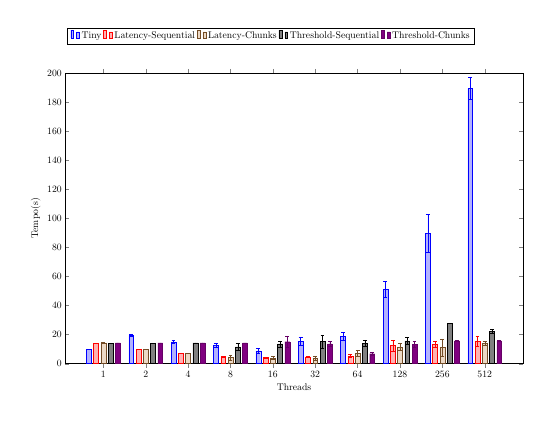
\begin{tikzpicture}[scale=0.35, baseline]
        \begin{axis}[
            width=1.5 \linewidth,
            height=1 \linewidth,
            %media de tempo intruder
            ybar=2.5pt,
            %enlargelimits=0.10,
            legend style={at={(0.45,1.1)}, anchor=south, legend columns=-1},
            ylabel=Tempo(s),
            xlabel=Threads,
            symbolic x coords={1, 2, 4, 8, 16, 32, 64, 128, 256, 512},
            xtick=data,
            ymin=0,
            ymax=200,
            bar width=5pt,
            % nodes near coords,
            nodes near coords align={vertical},
        ]
        \addplot+[error bars,y dir=both, y explicit] coordinates {
            (1,9.95)+-(1,0.09) (2,19.42)+-(2,0.50) (4,15.05)+-(4,1.07) (8,12.75)+-(8,1.30) (16,8.85)+-(16,1.90) (32,15.25)+-(32,2.69) (64,18.85)+-(64,2.74) (128,51.34)+-(128,5.50) (256,89.66)+-(256,12.90) (512,189.43)+-(512,7.63) 
        };
        \addplot+[error bars,y dir=both, y explicit] coordinates {
            (1,14.09)+-(1,0.09) (2,9.88)+-(2,0.04) (4,7.22)+-(4,0.04) (8,4.78)+-(8,0.29) (16,4.19)+-(16,0.35) (32,4.74)+-(32,0.50) (64,5.38)+-(64,1.21) (128,12.38)+-(128,3.72) (256,13.14)+-(256,2.01) (512,15.43)+-(512,3.54)
        };
        \addplot+[error bars,y dir=both, y explicit] coordinates {
            (1,14.31)+-(1,0.16) (2,9.98)+-(2,0.07) (4,7.23)+-(4,0.11) (8,4.19)+-(8,1.93) (16,3.85)+-(16,0.97) (32,3.96)+-(32,1.37) (64,7.11)+-(64,1.83) (128,11.47)+-(128,2.48) (256,11.12)+-(256,5.94) (512,14.17)+-(512,1.47)
        };
        \addplot+[error bars,y dir=both, y explicit] coordinates {
            (1,14.17)+-(1,0.05) (2,14.17)+-(2,0.11) (4,14.20)+-(4,0.08) (8,11.61)+-(8,2.13) (16,13.53)+-(16,1.93) (32,15.15)+-(32,4.48) (64,14.19)+-(64,2.00) (128,15.69)+-(128,2.21) (256,27.92)+-(256,0.20) (512,22.18)+-(512,1.28) 
        };
        \addplot+[error bars,y dir=both, y explicit] coordinates {
            (1,14.35)+-(1,0.05) (2,14.29)+-(2,0.04) (4,14.31)+-(4,0.08) (8,14.31)+-(8,0.05) (16,15.07)+-(16,4.06) (32,13.64)+-(32,1.83) (64,6.83)+-(64,1.09) (128,13.37)+-(128,2.19) (256,15.65)+-(256,0.16) (512,15.73)+-(512,0.14)
        };
        \legend {Tiny, Latency-Sequential, Latency-Chunks, Threshold-Sequential, Threshold-Chunks}
        \end{axis}
        \end{tikzpicture}
    }

    % \caption{Tempo de execução (s) em NUMA variando o número de \emph{threads}.}
    % \label{temp2}

\end{figure}
